\documentclass{article}
\usepackage[margin=10.5em]{geometry}
\usepackage{algorithm}
\usepackage{algorithmicx}
\usepackage{algpseudocode}
\usepackage{tikz}
\usepackage{tikz-qtree}
\setlength{\parskip}{\baselineskip}
\title{The Knapsack Problem \\ \small \textit{A Survey of Solution Approaches}}
\date{\small \today}
\author{Sayak Biswas \\ \small UNIVERSITY \textit{of} \textbf{FLORIDA} \\ \small UFID: 54584911}
\begin{document}
\pagenumbering{gobble}
\maketitle
\begin{abstract}
This paper surveys existing literature for different approaches to solve the knapsack problem. The Knapsack Problem is a combinatorial optimization problem in which one has to maximize the profits gained by packing a set of objects in a knapsack without exceeding its capacity. The problem is $\mathcal{NP}$-hard, thus there is no known polynomial time algorithm for a large input.

Specifically, we take a look at the \textit{0-1 Knapsack Problem} and provide a qualitative comparison between the two well-known approaches towards solving the problem: dynamic programming and backtracking algorithms.
\end{abstract}
\newpage

\pagenumbering{arabic}

\section{Introduction}
The \textit{Knapsack Problem} is an optimization problem, which at a high level is to choose the most profitable subset from a collection of available items without overloading the knapsack. The problem is formally defined as follows:

Given a knapsack of maximum capacity \textit{C} and \textit{n} items each weighing \textit{$w_{i}$} and with an associated profit of \textit{$p_{i}$}, the \textit{Knapsack Problem} is to choose a subset of the items such to maximize $\sum_{i=1}^{n}\textit{$p_{i}x_{i}$}$ on the condition $\sum_{i=1}^{n}\textit{$w_{i}x_{i}$} \leq \textit{C}, \textit{i} = 1,...,\textit{n}$ where \textit{$x_{i}$} is the number of copies of each item.

\iffalse
The \textit{fractional} knapsack problem allows placing a fraction \textit{$x_{i}$} of object \textit{i} into the knapsack \textit{i.e.} $0 \le \textit{$x_{i}$} \le 1$.

The \textit{bounded} knapsack problem restricts each item type to an integer amount of copies \textit{i.e.} \textit{$x_{i}$} $\in \{0,...,m_{i}\}$

The \textit{unbounded} knapsack problem removes any restriction from the number of copies of each object type \textit{i.e.} \textit{$x_{i}$} $\ge$ 0.
\fi

The \textit{0-1} knapsack problem restricts the copy count to either zero or one, meaning the object is either included in the knapsack or not, \textit{i.e.} \textit{$x_{i}$} $\in$ \{0, 1\}.

\section{Algorithms}
A na\"{\i}ve brute force approach would be to consider all $2^{n}$ possible combinations of items for the knapsack and choose the one that yields te maximum profit. Such an approach would lead to exponential complexity and hence is not desirable.
\subsection{Dynamic Programming}
Dynamic programming solves optimization problems by breaking it into smaller subproblems and then solving those subproblems to find the overall solution. \iffalse To solve a problem using dynamic programming, it should have two important characteristics:
\begin{itemize}
	\item \textit{Optimal Substructure}: This means that the overall optimal solution to a problem comprises optimal solutions to the subproblems.
	\item \textit{Overlapping Subproblems}: This means that any algorithm used to solve the problem should be solving a subset of the subproblems over and over again instead of generating new subproblems. Dynamic programming stores the results of these subproblems and uses them whenever the subproblem is encountered again. This is called \textit{memoization}.
\end{itemize}\fi
In this approach, we first define a function \textit{knap(1, n, C)} which finds the optimal solution, $f_{n}(C)$ for a knapsack of capacity \textit{C} using objects from \textit{1} to \textit{n}. We divide this into subproblems denoted by \textit{knap(1, j, y)} which finds the optimal solution for a knapsack of capacity \textit{y} using objects from \textit{1} to \textit{j}. Let the solution to this be defined by $f_{j}(y)$.

At any point in the problem state, the solution depends on making a decision on whether to use the current object or not. So, we obtain the top-down recurrence relation

\begin{equation} \label{eq:knapeq1}
	f_{j}(y) = max \quad \{f_{j-1}(y), f_{j-1}(y-w_{j}) + p_{j}\}, {y \ge w_{j}}
\end{equation}

Let us consider an example with a knapsack of capacity $C = 6$, three given objects with weights 2,3,4 and profits 1,2,5 respectively. Using the relation \ref{eq:knapeq1} we calculate all possible values and store them in a table as follows
\begin{center}
	\begin{tabular}{*8c}
		& 0 &1 &2 &3 &4 &5 &6 \\\cline{2-8}
		$f_{1}(y)$ &\multicolumn{1}{|c|}{0} &\multicolumn{1}{|c|}{0} &\multicolumn{1}{|c|}{1} &\multicolumn{1}{|c|}{1} &\multicolumn{1}{|c|}{1} &\multicolumn{1}{|c|}{1} &\multicolumn{1}{|c|}{1} \\\cline{2-8}
		$f_{2}(y)$ &\multicolumn{1}{|c|}{0} &\multicolumn{1}{|c|}{0} &\multicolumn{1}{|c|}{1} &\multicolumn{1}{|c|}{2} &\multicolumn{1}{|c|}{2} &\multicolumn{1}{|c|}{3} &\multicolumn{1}{|c|}{3} \\\cline{2-8}
		$f_{3}(y)$ &\multicolumn{1}{|c|}{0} &\multicolumn{1}{|c|}{0} &\multicolumn{1}{|c|}{1} &\multicolumn{1}{|c|}{2} &\multicolumn{1}{|c|}{5} &\multicolumn{1}{|c|}{5} &\multicolumn{1}{|c|}{6} \\\cline{2-8}
	\end{tabular}
\end{center}
So, we have a matrix of size \textit{n} x \textit{C} which we fill in row-wise manner as values in a row depend on the previous row values. The running time is \textit{O(nC)} and the space requirement is \textit{O(C)}. Below is the pseudo-code:

\begin{algorithm}
	\caption{DynamicKnapsack(\textit{p, w, n, C})}\label{dynamicKnapsack}
	\begin{algorithmic}[1]
		\For{$j$ from 0 to $C$}
			\State $result[0, j]\gets 0$
		\EndFor
		
		\For{$i$ from 1 to $n$}
			\For{$j$ from 0 to $C$}
				\If{$w[i-1] > j$}
					\State $result[i, j]\gets result[i-1, j]$
				\Else
					\State $result[i, j]\gets max(result[i-1, j], result[i-1, j-w[i-1]] + p[i-1])$
				\EndIf
			\EndFor
		\EndFor
	\end{algorithmic}
\end{algorithm}

\subsection{Backtracking}
A backtracking algorithm builds a set of possible solution all the while discarding any partial solution candidates which it determines to be not feasible. As discussed earlier the solution space for \textit{0-1} Knapsack problem consists of $2^{n}$ ways of assigning 0 or 1 to $x_{i}$. Below is a possible solution space when $n=3$.

\begin{center}
	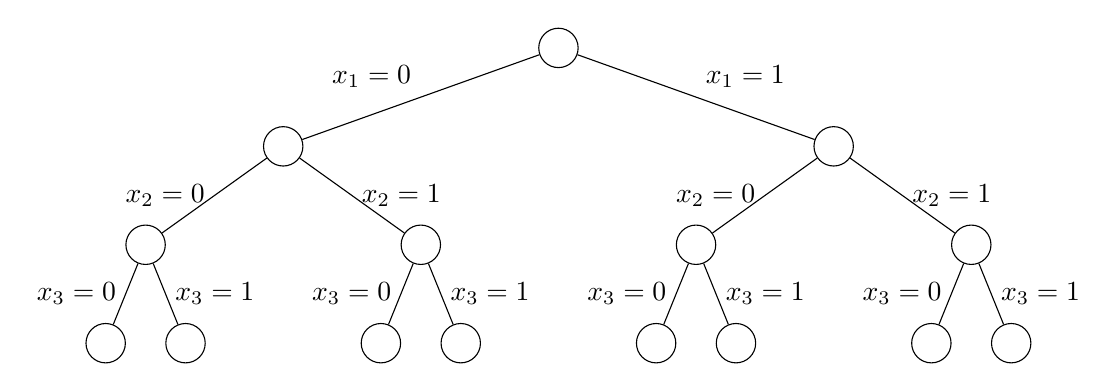
\begin{tikzpicture}[every tree node/.style={draw,circle},
		level distance=1.25cm, sibling distance=0.5cm, minimum size = 0.5cm,
		edge from parent path={(\tikzparentnode) -- (\tikzchildnode)}]
	\Tree
	[.{}
		\edge node[auto=right] {$x_{1} = 0$};
		[.{}
			\edge node[midway, left] {$x_{2} = 0$};
			[.{}
				\edge node[midway, left] {$x_{3} = 0$};
				[.{} ]
				\edge node[midway, right] {$x_{3} = 1$};
				[.{} ]
			]
			\edge node[midway, right] {$x_{2} = 1$};
			[.{}
				\edge node[midway, left] {$x_{3} = 0$};
				[.{} ]
				\edge node[midway, right] {$x_{3} = 1$};
				[.{} ]
			]
		]
		\edge node[auto=left] {$x_{1} = 1$};
		[.{}
			\edge node[midway, left] {$x_{2} = 0$};
			[.{}
				\edge node[midway, left] {$x_{3} = 0$};
				[.{} ]
				\edge node[midway, right] {$x_{3} = 1$};
				[.{} ]
			]
			\edge node[midway, right] {$x_{2} = 1$};
			[.{}
				\edge node[midway, left] {$x_{3} = 0$};
				[.{} ]
				\edge node[midway, right] {$x_{3} = 1$};
				[.{} ]
			]
		]
	]
	\end{tikzpicture}
\end{center}
This space is searched in depth-first manner from the start node. From each E-node we check if the next node will result in a feasible solution. If yes, the next node becomes the E-node. If no, we backtrack to the previous node and kill the E-node. To do this, we use an upper bound on the best solution that can be achieved from this node. We obtain this bound by relaxing the constraint from \textit{$x_{i}$} $\in$ \{0, 1\} to $0 \le \textit{$x_{i}$} \le 1$ and using the greedy algorithm (of sorting the items in non-decreasing order of profit per unit weight and adding to the knapsack) for the rest of the problem. The pseudo-code for the bounding algorithm and the backtracking solution is given below.
\begin{algorithm}
	\caption{GreedyBound(\textit{p, w, n, C, k, $p_{c}$, $w_{c}$})}\label{greedyBound}
	\begin{algorithmic}[1]
		\For{$i$ from $k+1$ to $n$}
			\State $w_{c} \gets w_{c} + w_{i}$
			\If{$w_{c} < C$}
				\State $p_{c} \gets p_{c} + p_{i}$
			\Else
				\State \Return $p_{c} + (1 - (w_{c} - C)/w_{i}) * p_{i}$
			\EndIf
		\EndFor
		\State \Return $p_{c}$
	\end{algorithmic}
\end{algorithm}

\begin{algorithm}
	\caption{BacktrackingKnapsack(\textit{p, w, n, C, k, $p_{c}$, $w_{c}$})}\label{backtrackingKnapsack}
	\begin{algorithmic}[1]
		\If{$w_{c} + w_{k} \le C$}
			\State $y_{k} \gets 1$
			\If{$k < n$}
				\State \Call{BacktrackingKnapsack}{\textit{p, w, n, C, k+1, $p_{c} + p_{k}$, $w_{c} + w_{k}$}}
			\EndIf
			\If{$p_{c} + p_{k} > p_{t}$ \textbf{and} $k=n$}
				\State $p_{t} \gets p_{c} + p_{k}$
				\State $w_{t} \gets w_{c} + w_{k}$
				\For{$j$ from 1 to $k$}
					\State $x_{j} \gets y_{j}$
				\EndFor
			\EndIf
		\EndIf
		\If{$\Call{GreedyBound}{\textit{p, w, n, C, k, $p_{c}$, $w_{c}$}} \ge p_{t}$}
			\State $y_{k} \gets 0$
			\If{$k < n$}
				\State \Call{BacktrackingKnapsack}{\textit{p, w, n, C, k+1, $p_{c}$, $w_{c}$}}
			\EndIf
			\If{$p_{c} > p_{t}$ \textbf{and} $k=n$}
				\State $p_{t} \gets p_{c}$
				\State $w_{t} \gets w_{c}$
				\For{$j$ from 1 to $k$}
					\State $x_{j} \gets y_{j}$
				\EndFor
			\EndIf
		\EndIf
		
	\end{algorithmic}		
\end{algorithm}

\section{Qualitative Comparison}
As we saw above, the brute force approach has a complexity of \textit{O(n$2^{n}$)}. Although it is quite simple to code, it can be used only for very small input due to its exponential complexity. 

The dynamic programming approach performs much better with a running time of \textit{O(nC)}. It also has a space complexity of \textit{O(C)}. This stems from the fact that in a dynamic programming approach we need to store two rows of a \textit{C}-column array as values in the current row are calculated using those from the previous row. From the perspective of coding complexity, it is also quite easy to implement.

The backtracking algorithm will create the complete state space tree with $2^{n-1}-1$ nodes in the worst case. In theory it is hard to say how much of the search tree is pruned out by the bounding heuristics however in practice it does not generate all the possible nodes, so there is a substantial speed increase. The implementation in code is a bit more difficult in this case compared to the dynamic programming method.

\section{Conclusion}
In this paper we looked at two approaches to solve the \textit{0-1} Knapsack problem. We saw that runtimes for both the approaches have different characteristics. As such it cannot be explicitly defined which algorithm is a better choice. This needs to be determined by implementing both algorithms and executing the code by varying the input number of items and the maximum capacity of the knapsack.

\section{References}
Horowitz, Ellis and Sahni, Sartaj and Rajasekaran, Sanguthevar, 2007, \textit{Computer Algorithms}, Silicon Pr., 773p

\end{document}